\section{Evaluation}
\label{sec:evaluation}



We present a comprehensive evaluation of \tool, structured around the following research questions:

\begin{itemize}
    \item \textbf{RQ1 (Detection Effectiveness).}
          How accurately does \tool match prompt injection attacks across systematically generated adversarial variants, from simple word substitutions to comprehensive semantic paraphrasing, compared to the SimHash~\cite{manku2007detecting} baseline?

    \item \textbf{RQ2 (Privacy-Utility Trade-off).} What is the quantitative relationship between \tool's randomized response mechanism ($\alpha$) and threat detection utility?

    \item \textbf{RQ3 (Noise Calibration \& Predictability).} Does the empirical self-Hamming distortion introduced by randomized response match the theoretical $(1-p)d$ curve across $\alpha$, letting us confidently choose a privacy setting?

    \item \textbf{RQ4 (Scalability).} Does \tool maintain consistent detection accuracy as corpus size scales from thousands to hundreds of thousands of entries, reflecting realistic enterprise deployment scenarios where malicious prompts are sparse within benign prompts?

    \item \textbf{RQ5 (Computational Efficiency).} What are the computational gains of \tool's fingerprints compared to dense embeddings, and do these improvements enable practical real-time threat correlation at enterprise scale?

\end{itemize}

\subsection{Evaluation Settings}

\subsubsection{Datasets}
We evaluate \tool using the recent prompt injection dataset from \cite{shen2024doanything}, which contains real-world attack and benign prompts. From this, we construct a comprehensive evaluation set simulating adversarial scenarios, enabling controlled and realistic assessment of threat intelligence. 

Given the inherent challenge of obtaining large-scale labeled datasets of semantically similar prompt injection variants, we develop a systematic methodology for generating controlled attack modifications to validate threat intelligence.
Our synthetic data generation process creates two primary types of variants: \emph{Word-Flipping Variants:} For each adversarial prompt, we randomly select $x$ words (where $x \in \{1, 3, 5, 10, 20\}$) longer than four characters and replace them with semantically equivalent synonyms using GPT-4o.
This simulates subtle adversarial modifications that maintain attack intent while altering surface-level tokens.
The language model is guided using the structured prompt listed in Appendix~\Cref{prompt:words-flipped}.
\emph{Paraphrase Variants:} We generate comprehensive paraphrased versions of prompts using GPT-4o while preserving the underlying attack intent. 
Appendix~\Cref{prompt:paraphrase} contains the prompt.
\emph{Benign Pairs:} Benign prompts are systematically paired such that each pair consists of two semantically unrelated prompts, ensuring they serve as appropriate negative examples for similarity detection algorithms (e.g., SimHash and \tool).
%
The resulting dataset undergoes rigorous filtering to ensure quality and consistency (e.g., remove duplicates, empty prompts).
The final dataset is balanced with equal numbers of attack and benign pairs, with attack pairs labeled as 1 and benign pairs labeled as 0.
This balanced approach ensures unbiased evaluation across both positive and negative cases.
%
Our synthetic generation methodology enables systematic evaluation across varying levels of attack sophistication, from minimal single-word modifications to comprehensive paraphrasing.

\subsubsection{Baseline}

Our evaluation compares \tool against SimHash~\cite{manku2007detecting}, a widely-adopted locality-sensitive hashing baseline.
\tool operates by first extracting semantic features using an embedding model. 
To demonstrate its flexibility with both open-source and proprietary options, we evaluate \tool using ModernBert~\cite{gill2025advancingsemanticcachingllms} and an OpenAI model. 



\subsubsection{Evaluation Metrics}
We employ a comprehensive set of metrics to assess both detection performance and privacy-utility tradeoffs. For detection performance, we use precision, recall, accuracy, and F1-score across varying similarity thresholds to evaluate attack detection accuracy. Threshold analysis is performed using precision-recall curves to identify the optimal threshold for Hamming distance and to understand how performance is affected by threshold selection, as discussed in~\cite{manku2007detecting}. We also include confusion matrices for detailed analysis of true positives (TP), false positives (FP), true negatives (TN), and false negatives (FN) at optimal thresholds.

\begin{figure}[t]
    \begin{subfigure}[b]{0.45\textwidth}
        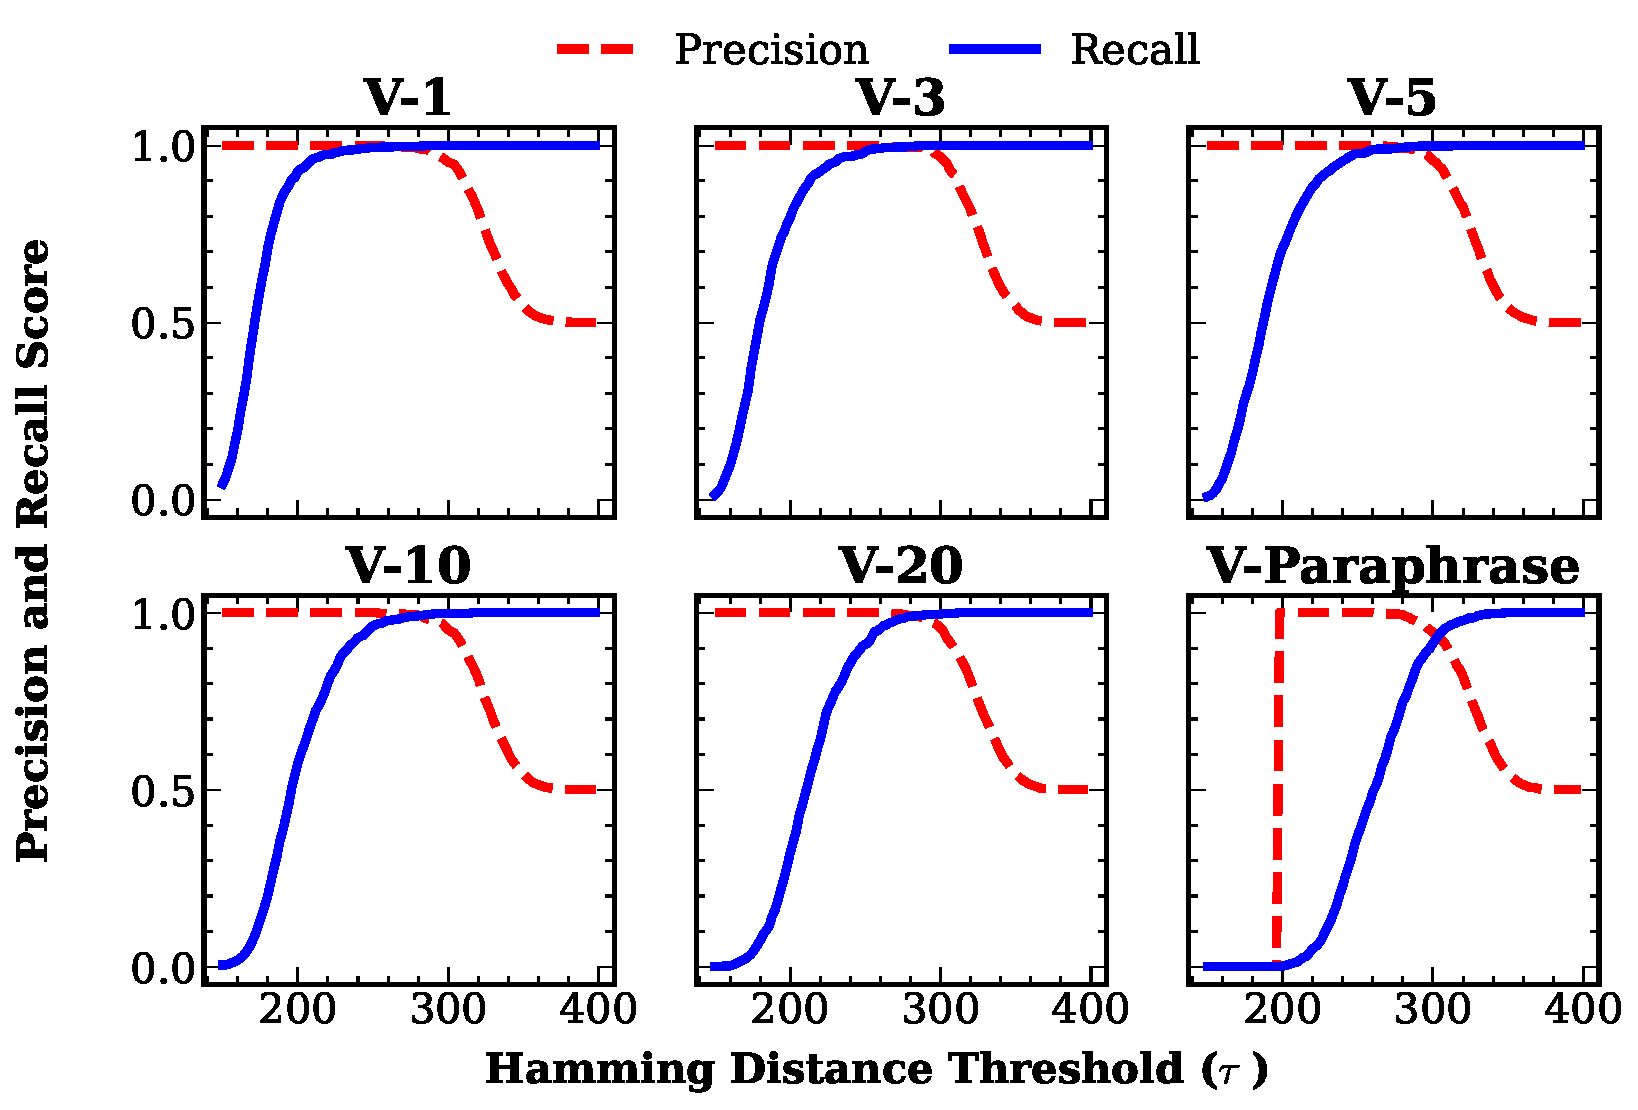
\includegraphics[width=\textwidth]{exp_results/BinaryShield/BinaryShield_precision_recall_curves.pdf}
        \caption{Precision-recall curves across attack variants.}
        \label{fig:binaryshield_pr}
    \end{subfigure}
    \hfill % small manual gap (adjust or remove)
    \begin{subfigure}[b]{0.45\textwidth}
        \centering
            \centering
            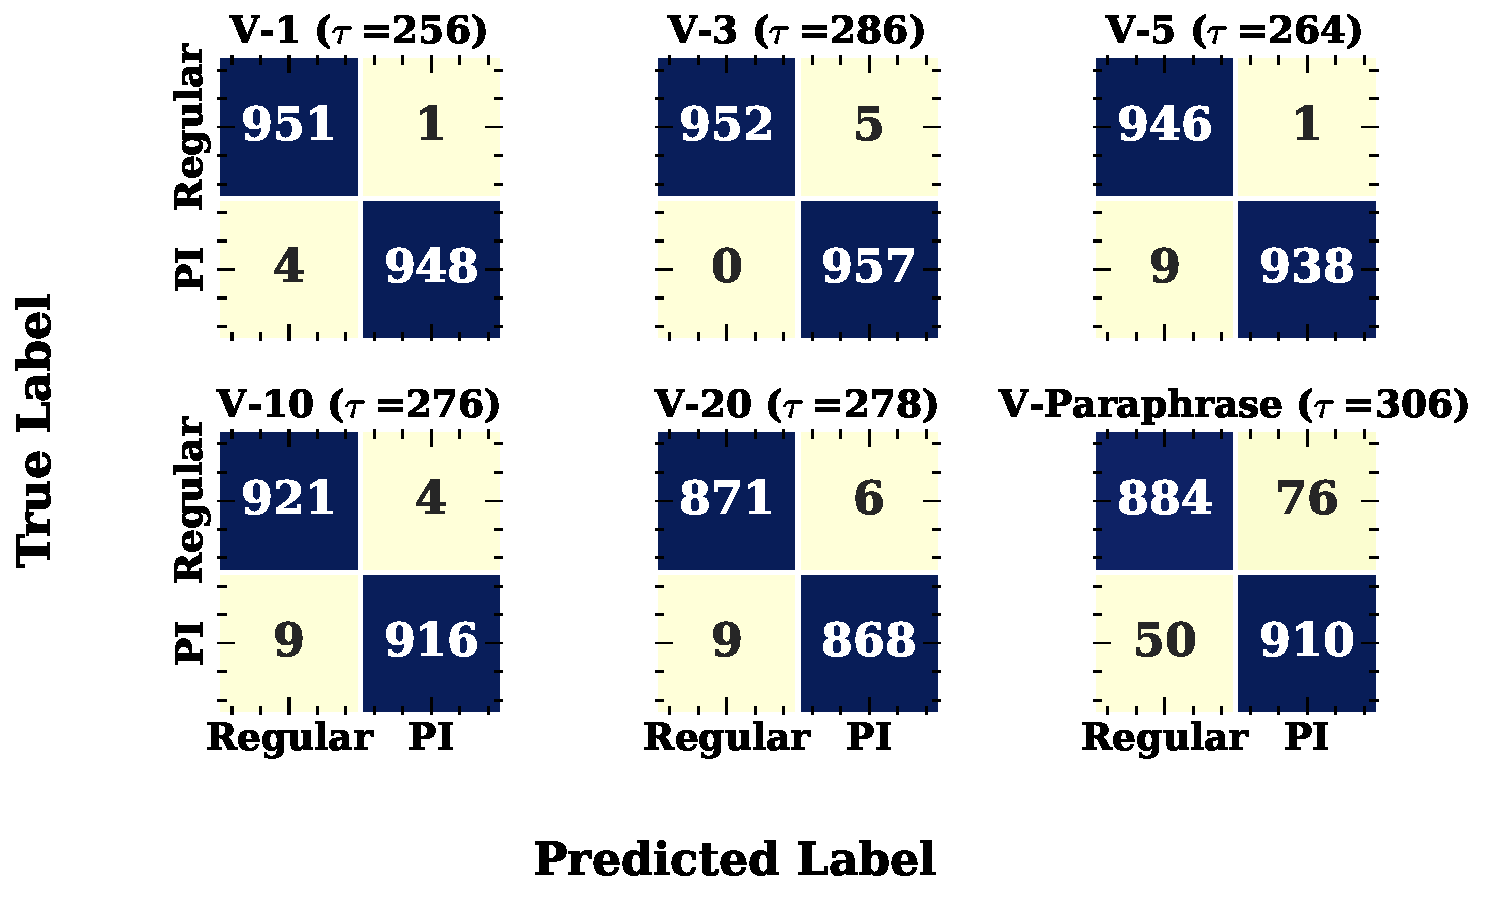
\includegraphics[width=\linewidth]{exp_results/BinaryShield/BinaryShield_confusion_matrices.pdf}
        \caption{Confusion matrices at optimal thresholds.}
        \label{fig:binaryshield_cm}
    \end{subfigure}
    \caption{\underline{\textbf{\tool}} performance analysis across attack variants with $\alpha = 2.0$. (a) Precision-recall curves demonstrate consistent performance across variants. (b) Confusion matrices at optimal Hamming distance thresholds show TP, TN, FP, and FN counts, indicating strong detection capabilities even under complex paraphrasing attacks. Note that \textbf{PI} in the confusion matrices stands for \emph{Prompt Injection} and is used to distinguish between attack and benign prompts.}
    \label{fig:binaryshield_results}
    \vspace{-4mm}  
\end{figure}

\begin{figure}[t]
    \centering
    \begin{subfigure}[b]{0.45\textwidth}
        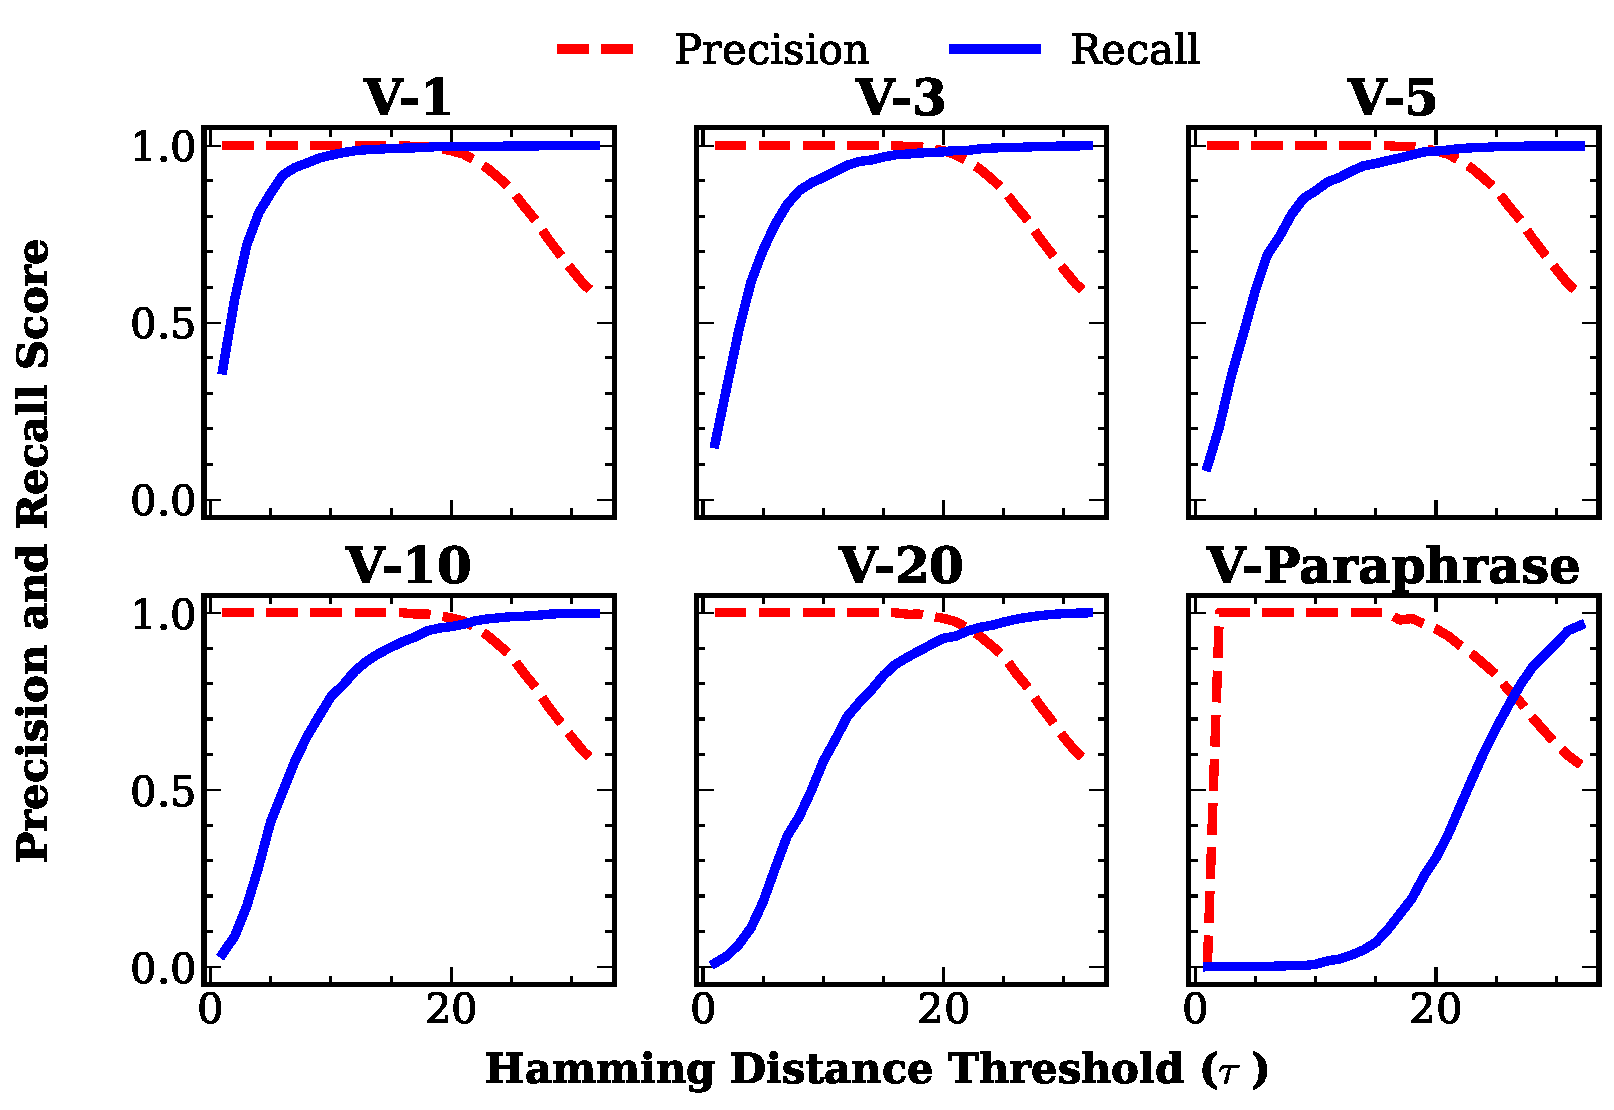
\includegraphics[width=\textwidth]{exp_results/SimHash/SimHash_precision_recall_curves.pdf}
        \caption{Precision-recall curves across attack variants.}
        \label{fig:simhash_pr}
    \end{subfigure}
    \hfill
    \begin{subfigure}[b]{0.45\textwidth}
            \centering
            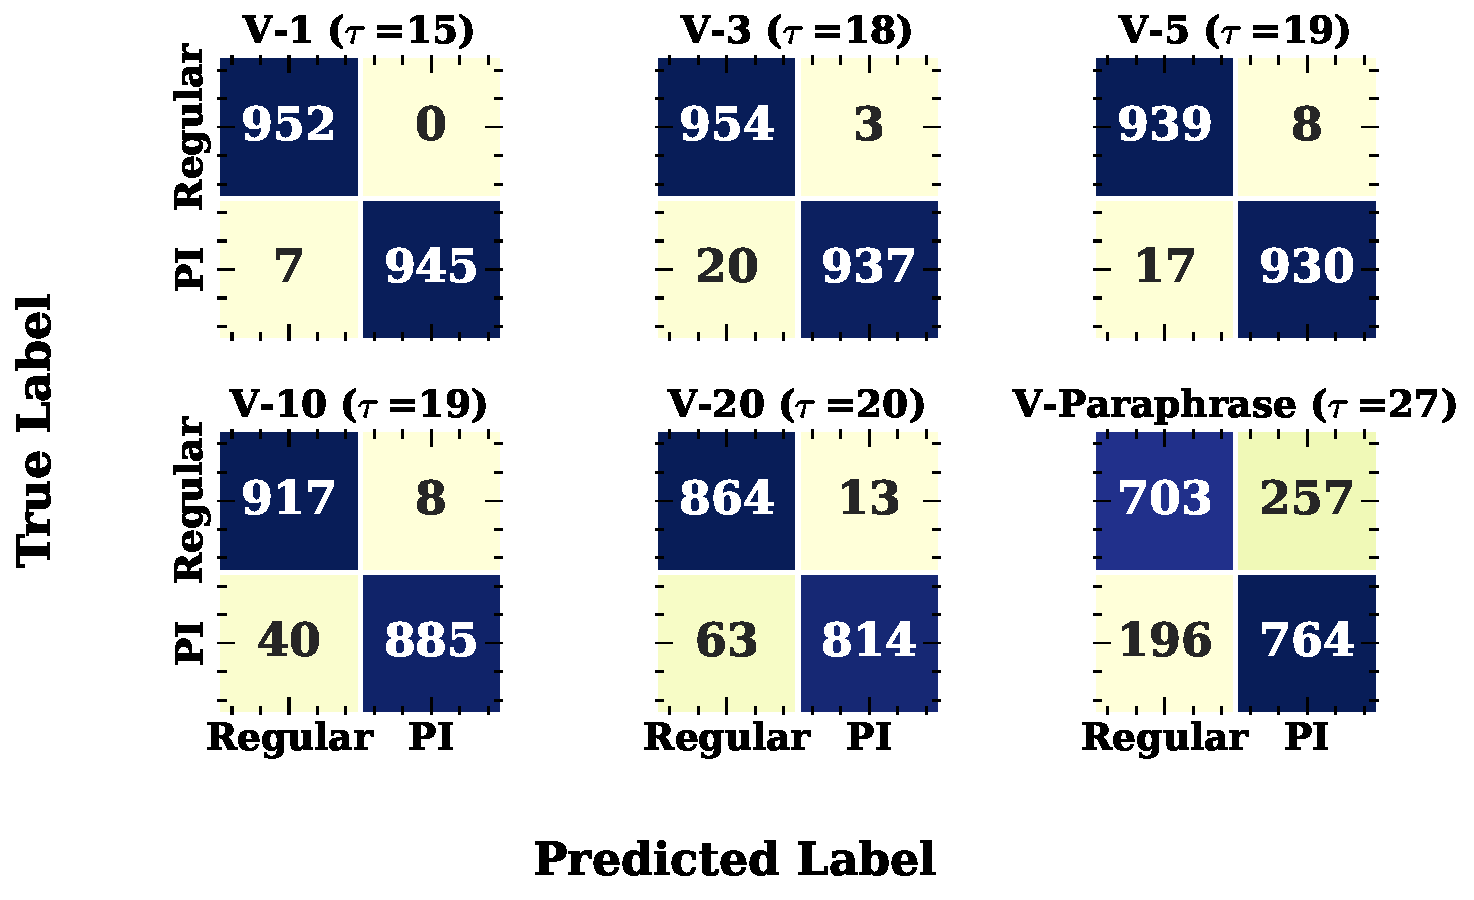
\includegraphics[width=\textwidth]{exp_results/SimHash/SimHash_confusion_matrices.pdf}
        \caption{Confusion matrices at optimal thresholds.}
        \label{fig:simhash_cm}
    \end{subfigure}
    \caption{\underline{\textbf{SimHash}} baseline performance analysis across attack variants. Confusion matrices reveal growing FP and FN, particularly for paraphrasing scenarios.}
    \label{fig:simhash_results}
    \vspace{-4mm}  
\end{figure}

\subsection{\tool Comparison with Baseline}
\label{sec:comparison-baseline}

To provide a rigorous performance analysis, we systematically compare \tool against SimHash, a widely used locality-sensitive semantic hashing method~\cite{manku2007detecting}.
Both algorithms generate binary fingerprints and use Hamming distance for similarity measurement, making them directly comparable.
This baseline is chosen to evaluate not only detection performance but also the privacy-preserving capabilities essential for cross-boundary threat intelligence sharing as SimHash also generates privacy-preserving binary fingerprints.



For this \emph{evaluation}, we configure \tool with a differential privacy parameter of $\alpha = 2.0$, which provides meaningful privacy protection while maintaining strong detection performance.
Our comparative analysis encompasses six distinct attack variants: minimal single-word modifications (V-1), progressive word changes (V-5, V-20) and extensive modifications in paraphrasing scenarios (V-Paraphrase) that fundamentally restructure prompts while preserving malicious intent.
This progression allows us to assess how each method's performance degrades as attack sophistication increases during threat correlation.
Figure~\ref{fig:binaryshield_results} and Figure~\ref{fig:simhash_results} present comprehensive performance analysis through precision-recall curves and confusion matrices at optimal operating points.
\begin{figure}
    \centering
    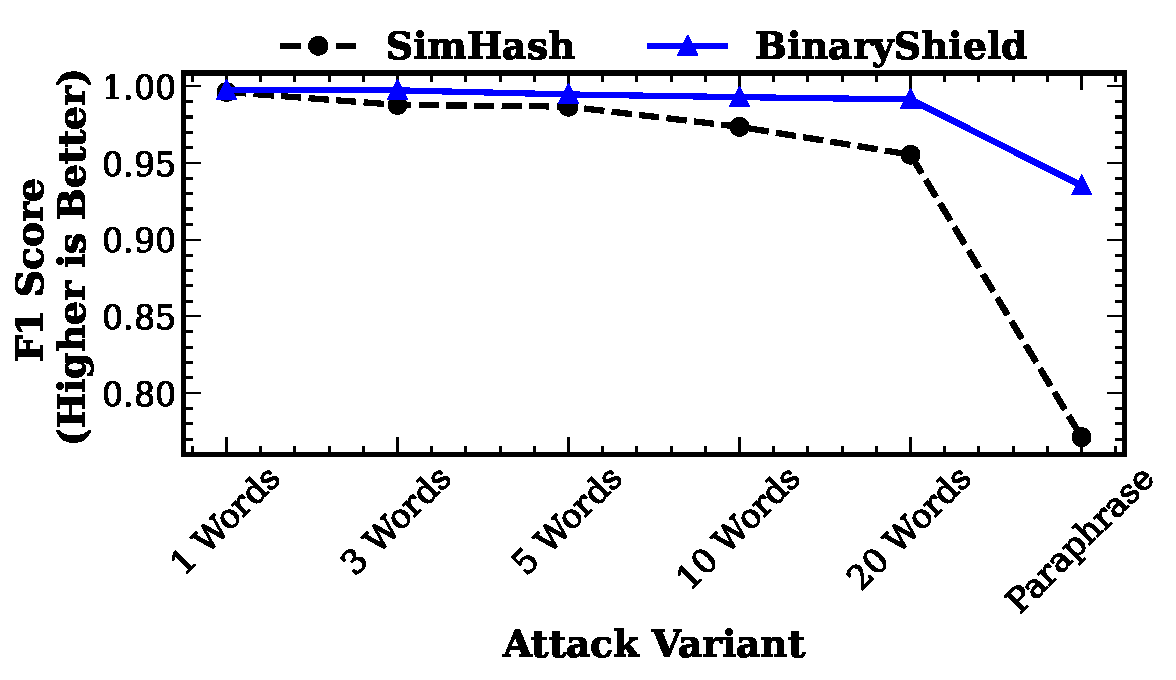
\includegraphics[width=0.75\linewidth]{exp_results/comparisons/simhash_vs_binaryshield_f1_comparison.pdf}
    \caption{F1-score comparison between \tool and SimHash across attack variants. \tool outperforms SimHash, particularly in complex paraphrasing scenarios, demonstrating superior robustness to semantic modifications.}
    \label{fig:simhash_vs_binaryshield_f1}
    \vspace{-4mm}  
\end{figure}

For minimal attack modifications (V-1 to V-10), both algorithms demonstrate exceptional detection capabilities with near-perfect performance (Figure~\ref{fig:simhash_vs_binaryshield_f1}).
At optimal thresholds, both methods achieve optimal F1-scores (Figure~\ref{fig:simhash_vs_binaryshield_f1}), establishing a strong baseline for more complex evaluations.
For instance, in the V-10 scenario, SimHash produces 8 false positives and 40 false negatives at Hamming distance threshold ($\tau$) 19 (Figure~\ref{fig:simhash_results}), while \tool generates only 4 false positives at threshold 276 (Figure~\ref{fig:binaryshield_results}).

As attack complexity increases to extensive word modifications (V-20), performance differences begin to emerge.
\tool maintains robust performance with an F1-score of 0.99 (precision: 0.99, recall: 0.98), while SimHash experiences measurable degradation to an F1-score of 0.96 (precision: 0.98, recall: 0.93).
The 3.3\% gap starts to illustrate \tool's superior stability as lexical modifications increase.

The most challenging scenario involves comprehensive paraphrasing attacks (V-Paraphrase), where prompts undergo fundamental restructuring while preserving malicious intent.
Here, the performance differential becomes most pronounced: \tool achieves an F1-score of 0.94 (precision: 0.92, recall: 0.95), while SimHash degrades significantly to an F1-score of 0.77 (precision: 0.75, recall: 0.80). This 17\% gap in F1 score demonstrates \tool's fundamental advantage in threat intelligence that transcends surface-level linguistic variations.

Additionally, examining \emph{confusion matrices} at optimal thresholds, provides additional insights into error patterns in Figures ~\ref{fig:binaryshield_cm} and ~\ref{fig:simhash_cm}. \tool demonstrates consistent performance as compared to SimHash. SimHash shows increasing error variability as attack complexity increases, struggling particularly to distinguish between semantically similar malicious content and unrelated benign prompts.
The 17 percentage point F1-score gap in paraphrasing attacks, the most challenging and operationally relevant scenario, validates the effectiveness of \tool.
These performance improvements are achieved while simultaneously providing privacy guarantees essential for cross-service threat intelligence. 


\begin{tcolorbox}[colback=white, colframe=black,  left=0pt, right=0pt, top=0pt, bottom=0pt]
    \textbf{Summary.}\ \tool consistently outperforms SimHash in threat correlation, especially under complex paraphrasing attacks, achieving an F1-score of 0.94 compared to SimHash's 0.77. These results highlight \tool's superior robustness with enabling privacy, making it highly effective for cross-service threat intelligence.
\end{tcolorbox}

\begin{figure}[t]
    \centering
    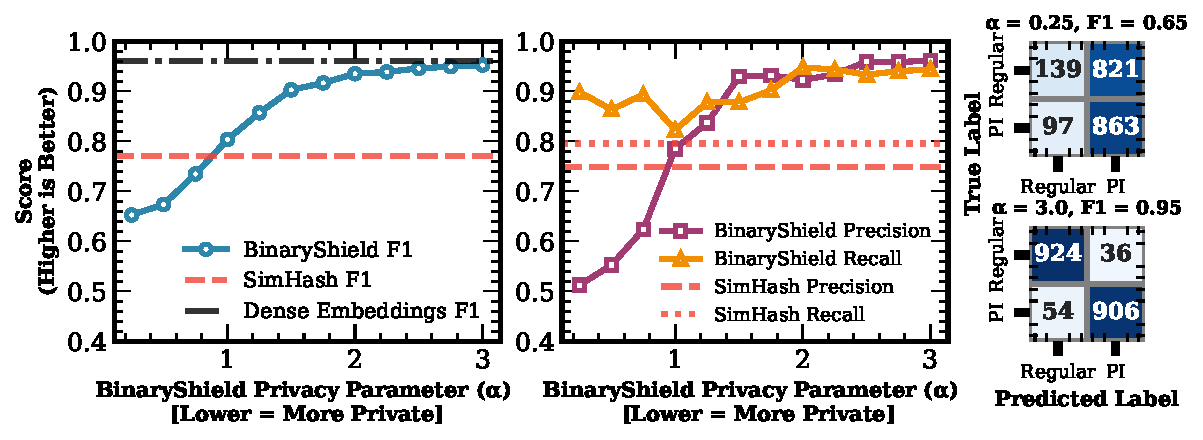
\includegraphics[width=\linewidth]{exp_results/epsilon_analysis/comprehensive_dp_analysis.pdf}
    \caption{Privacy-utility trade-off for paraphrased prompt injection detection. (Left) \tool F1 rises smoothly with privacy budget $\alpha$, dominating SimHash (privacy-preserving baseline) across most of the spectrum and approaching non-private dense embeddings. (Center) Precision lags recall at high noise, then rapidly converges after $\alpha\!\approx\!1$ as FP collapse. Horizontal dashed lines: SimHash precision/recall. (Right) Confusion matrices at extreme settings: severe noise ($\alpha=0.25$) induces many FP; higher $\alpha$ ($3$) sharply improves precision.}
    \label{fig:binaryshield-privacy-utility-tradeoff-with-baselines}
    \vspace{-4mm}  
\end{figure}

\subsubsection{Empirical Analysis of Randomized Response Impact}
\label{sec:empirical-randomized-response}

We quantify the impact of randomized response mechanism~\cite{warner1965randomized} noise on detection utility by sweeping the per‑bit privacy budget $\alpha\!\in\![0.25,3.0]$ (Algorithm~\ref{alg:binaryshield-pipeline}, Step 4) on the most challenging paraphrase attack variant.
For each $\alpha$, a bit in the 768‑dimensional binary embedding is kept with probability $p=\tfrac{e^{\alpha}}{e^{\alpha}+1}$ and flipped otherwise, yielding an expected self‑Hamming distortion $(1-p)d$, where $d$ is the fingerprint dimension (here, $d=768$).
At $\alpha=0.25$, $p=0.562$ and the mechanism flips $\approx0.438\times768\approx336$ bits (i.e., the whole binary vector is approximately completely randomized).
As shown in the top-right confusion matrix of Figure~\ref{fig:binaryshield-privacy-utility-tradeoff-with-baselines}, at this extreme privacy setting there are 821 false positives and 97 false negatives, resulting in an F1-score of only 0.65.
Such high noise levels provide maximal privacy but render the binary fingerprints nearly random (Figure~\ref{fig:binaryshield-noise-calibration}), offering little practical utility for threat detection.



Figure~\ref{fig:binaryshield-privacy-utility-tradeoff-with-baselines} shows that utility improves smoothly with larger $\alpha$ as noise shrinks.
At $\alpha=1.0$ precision increases to 0.79 with high recall of 0.82.
The inflection region $\alpha\!\in\![1.25,1.75]$ marks the transition where precision catches up to recall: by $\alpha=1.5$ \tool attains F1=0.90, already exceeding SimHash’s paraphrase F1 (0.77) by +13 points while providing privacy that is absent in dense cosine embeddings.
From $\alpha=2.5$ onward the F1 curve is close to the dense embeddings while still providing privacy as bit flipping probability is not zero (Figure~\ref{fig:binaryshield-noise-calibration}).
The confusion matrices at the privacy extremes (Figure~\ref{fig:binaryshield-privacy-utility-tradeoff-with-baselines}, right) illustrate this shift: moving from $\alpha=0.25$ to $3.0$ reduces false positives 22.8$\times$ (821$\rightarrow$36) and false negatives (97$\rightarrow$54), yielding an approximately 30‑point F1 gain (0.65$\rightarrow$0.95).
This predictable performance curve lets operators easily adjust $\alpha$ to meet privacy requirements, estimate detection accuracy, and securely share threat intelligence without revealing raw prompts or embeddings.

\noindent{\textbf{Randomized Response and Hamming Distance.}} To empirically validate \tool's privacy model, we conducted a controlled experiment measuring the actual Hamming distance introduced by the \tool's differential privacy.

To this end, for 500 prompts from our evaluation dataset, \tool generated 768-dimensional binary fingerprints and applied its differential privacy transformation by varying $\alpha$ values from 0.2 to 3.4.
For each configuration, we computed the Hamming distance between original and noise-perturbed fingerprints, comparing observed distances against the theoretical expectation $(1-p)d$.
As a baseline reference, we generated 1,000 pairs of independent random binary vectors to establish the average distance for completely uncorrelated binary vectors. The mean Hamming distance for these independent vectors is $384.44 \pm 13.65$, which serves as a baseline for comparison.
Figure~\ref{fig:binaryshield-noise-calibration} demonstrates that our theoretical model precisely predicts the observed self-Hamming distortion across all privacy levels confirming \tool's alignment with theory. At $\alpha = 0.2$, \tool's perturbed binary fingerprint reaches a Hamming distance of $346 \pm 13.41$, nearly matching the random baseline. This results in lower F1 scores at small $\alpha$ (Figure~\ref{fig:binaryshield-privacy-utility-tradeoff-with-baselines}).

\begin{figure}
    \centering
    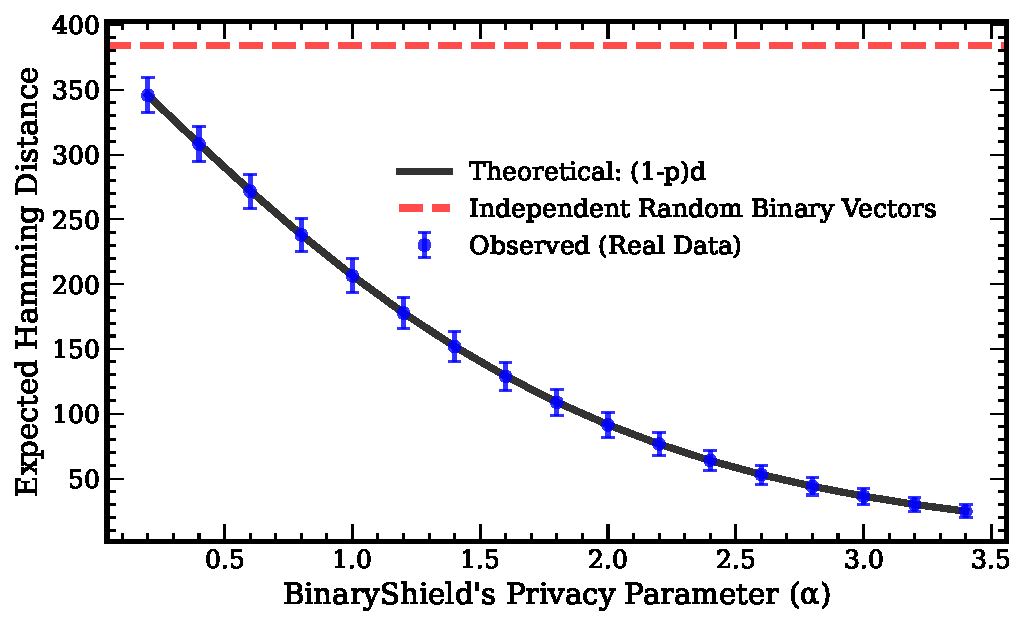
\includegraphics[width=0.7\linewidth]{exp_results/epsilon_analysis/BinaryShield_noise_vs_hamming_distance.pdf}
    \caption{Calibration of randomized-response noise. Empirical mean Hamming distances (blue points, $n=500$ each) between original and privatized 768-bit fingerprints tightly follow the theoretical curve $(1-p)d$ (solid black) across privacy budgets $\alpha$.
        The dashed red line shows the mean distance between independent random binary vectors (384), illustrating how increasing $\alpha$ moves \tool smoothly from near-randomization to low-distortion states.}
    \label{fig:binaryshield-noise-calibration}
    \vspace{-20pt} % tighten top if needed
\end{figure}

    




As $\alpha$ increases, the Hamming distance decreases to $206.45 \pm 13.08 $ at $\alpha = 1.0$. This decay directly correlates with the smooth utility recovery in Figure~\ref{fig:binaryshield-privacy-utility-tradeoff-with-baselines}.
The tight correspondence between theoretical predictions and observed measurements validates that \tool's privacy mechanism operates exactly as designed, providing operators with precise control over the privacy-utility trade-off through a single, well-characterized parameter $\alpha$.
Another noticeable observation is that even at higher $\alpha$ values, as shown in Figure~\ref{fig:binaryshield-noise-calibration}, the Hamming distance remains nonzero. This indicates that \tool continues to provide privacy protection, since the nonzero Hamming distance ensures privacy is maintained, even as its utility approaches that of dense embeddings (Figure~\ref{fig:binaryshield-privacy-utility-tradeoff-with-baselines} and~\ref{fig:binaryshield-noise-calibration}).
In contrast, dense embeddings offer no privacy at all, so even a nonzero Hamming distance (i.e., some privacy) is fundamentally better than nothing, ensuring that sensitive information is not directly exposed.

\begin{tcolorbox}[colback=white, colframe=black,  left=0pt, right=0pt, top=0pt, bottom=0pt]
    \textbf{Summary.}\ \tool exhibits the fundamental differential privacy trade-off: low $\alpha$ (strong privacy) yields near-random fingerprints, whereas increasing $\alpha$ (meaningful privacy) produces a smooth, monotonic F1 rise that quickly approaches non-private baseline performance.
\end{tcolorbox}

%% ===================================== Real-World Scenario Analysis =====================================

\begin{figure*}
    \centering
    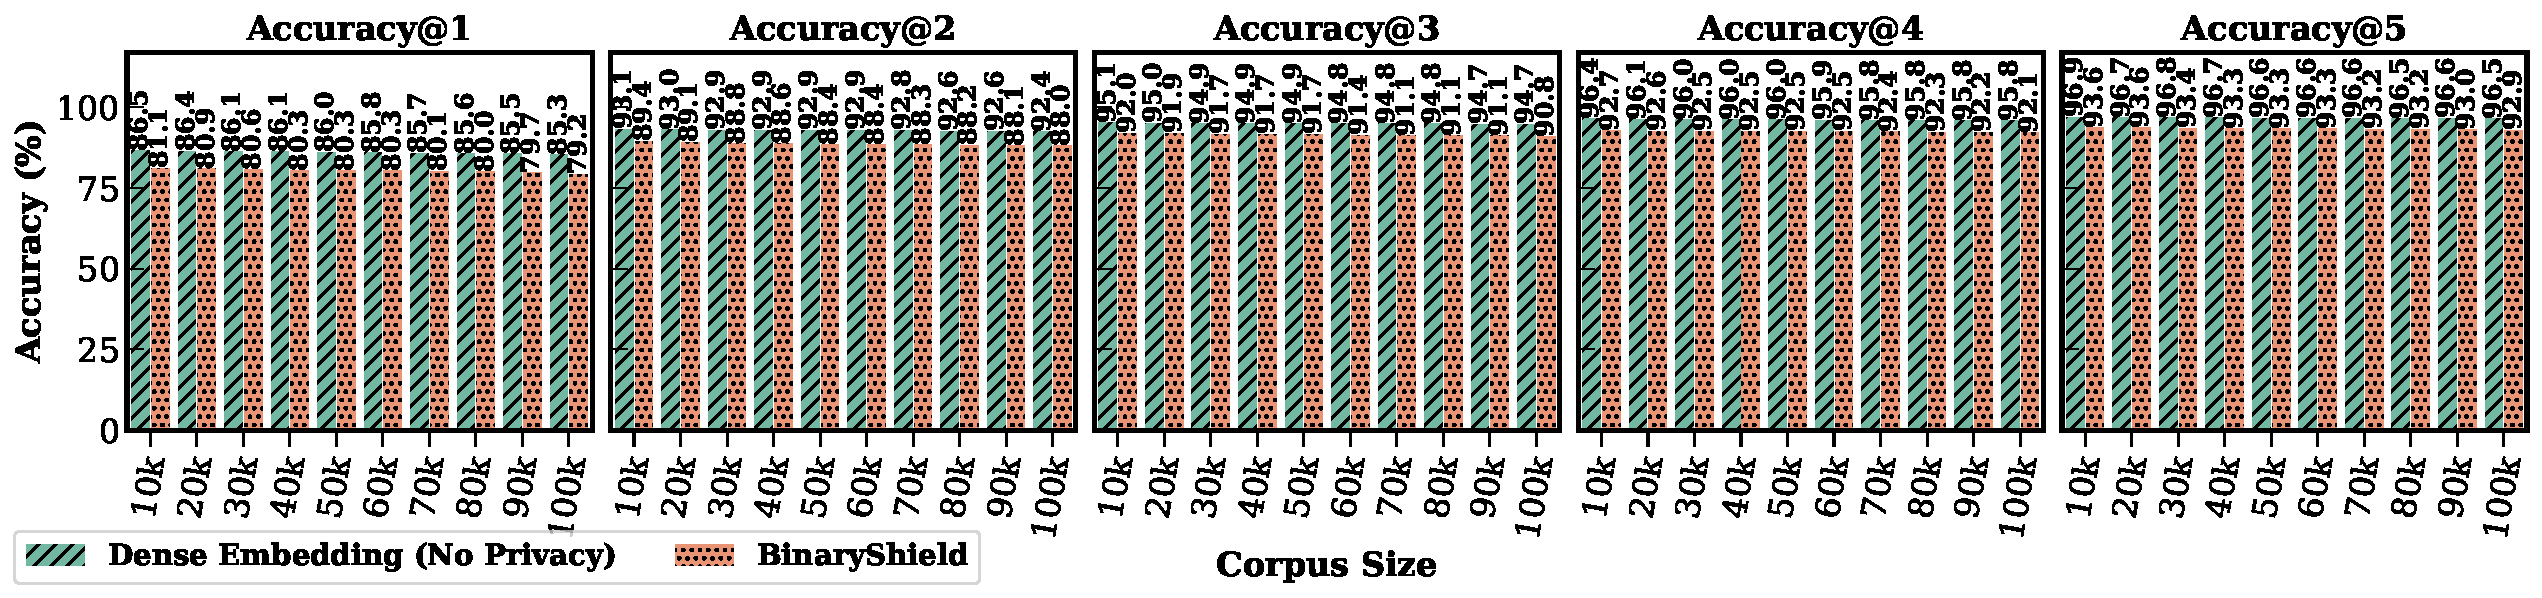
\includegraphics[width=\linewidth]{exp_results/real-world-scenario-results/accuracy_k_scalability_hybrid.pdf}
    \caption{Scalability of \tool.
        Accuracy@k for \tool vs \emph{non-private} dense embeddings baseline across hybrid corpora (10K-100K). \tool retains 93\% of baseline Accuracy@1 while providing privacy.}
    \label{fig:hybrid-accuracy-scalability}
    \vspace{-4mm}  
\end{figure*}

\subsection{Real-World Deployment Analysis}
\label{sec:real-world-analysis}

While earlier sections validate \tool's superior performance as compared to the privacy-preserving baseline (SimHash), we now turn to evaluating \tool's effectiveness in realistic cross-service threat intelligence scenarios.
Specifically, it must be shown that privacy-preserving correlation remains effective when (i) malicious prompts are sparse relative to benign traffic and (ii) corpus size scales by an order of magnitude  (iii) privacy-utility trade-off is maintained, i.e., the accuracy gap between \tool and non-private dense embeddings remains bounded, and (iv) efficiency is maintained in terms of computational and storage overhead.





\subsubsection{Large-Scale Threat Intelligence Scalability}
\label{sec:large-scale-threat-intelligence-scalability}
To simulate realistic enterprise conditions, we query attack fingerprints against corpora where benign prompts vastly outnumber malicious ones, measuring Accuracy@k as successful detection when the true variant ranks within the top-k retrieved candidates. The goal is to quantify how \tool's privacy-preserving fingerprint correlation accuracy behaves as the total corpus grows, and characterize the accuracy gap relative to a non-private dense embedding baseline. In this experiment, \tool uses OpenAI's  \texttt{text-embedding-3-large} to generate embeddings. 

We study this setting using hybrid corpora that interleave a (fixed) malicious prompt injection (\texttt{V-Paraphrase}) with large volumes of real user interactions from WildChat~\cite{zhao2024wildchat}, thereby emulating an enterprise log in which only a small fraction of entries are attacks. For each target corpus size $C \in \{10\text{K},20\text{K},\dots,100\text{K}\}$, we construct a hybrid dataset by injecting a fixed malicious prompt set into $C - M$ benign WildChat prompts (where $M$ is the number of distinct attack prompts).
Each malicious prompt is issued as a query; success is recorded if its exact counterpart (or semantically identical variant, depending on $k$) appears within the top-$k$ candidates when ranked by Hamming distance over \tool's fingerprints, or cosine similarity for the dense baseline. We fix the local differential privacy parameter at $\alpha = 2$ (different $\alpha$ values are also evaluated in Section~\ref{sec:scalability-privacy-utility}).

Figure~\ref{fig:hybrid-accuracy-scalability} shows the results of threat intelligence scalability analysis, with the X-axis showing corpus sizes (10K to 100K) and the Y-axis representing retrieval accuracy.
\emph{Accuracy@k represents the percentage of queries for which the correct malicious prompt is returned in the first k-results.}
Accuracy@1 for the dense baseline declines modestly by only 1.2\% points across a 10$\times$ increase in corpus size (86.5\% $\rightarrow$ 85.3\%).
\tool{} shows a similarly shallow decline (81.1\% $\rightarrow$ 79.2\%; 1.9\% points). This indicates that neither binary quantization nor randomized response mechanism introduces scale-sensitive degradation.

Furthermore,~\Cref{fig:hybrid-accuracy-gap} (in the appendix) shows that the Accuracy@k \emph{gaps} between \tool and the dense baseline with X-axis showing corpus sizes (10K to 100K) and Y-axis showing the gap at different top-k accuracy.
The gap remains tightly bounded: it ranges from 5.31\% to 6.15\% (mean 5.66\% points) at $k=1$, indicating that \tool retains over 93\% of the dense baseline's accuracy even under tight local differential privacy constraints.
Crucially, the gap does \emph{not} significantly widen with corpus size.
Furthermore, increasing $k$ rapidly closes the gap, as shown in Figure~\ref{fig:hybrid-accuracy-scalability} and Figure~\ref{fig:hybrid-accuracy-gap}.
For instance at 100K entries, \tool achieves 79.2\% Accuracy@1, 90.8\% Accuracy@3, and 92.9\% Accuracy@5. On the same 100K corpus, the dense embeddings achieve 85.3\% Accuracy@1, 94.7\% Accuracy@3, and 96.5\% Accuracy@5.
The gap at $k=5$ is only 3.6\% points, indicating that \tool's with  privacy feature reaches close to the \emph{non-private} baseline of dense embeddings.
This confirms that the semantic signal preserved after (i) sign-only quantization and (ii) per-bit randomized response still remains sufficiently rich for practical threat correlation.
For every corpus size, \tool's incremental gains from $k=1$ to $k=2$ average roughly +8\% (Figure~\ref{fig:hybrid-accuracy-scalability}).
This reflects that most residual misses at $k=1$ are near-boundary semantic neighbors retrievable with minimal expansion. Subsequent marginal gains ($k>2$) diminish smoothly.
Figure~\ref{fig:hybrid-accuracy-gap} shows the gap curves monotonically compress as $k$ increases.
The gap is attributable to two irreversible transformations: (a) many-to-one sign mapping (loss of magnitude information) and (b) randomized response bit flips calibrated by $\alpha=2$.
That the gap does not drift upward with scale empirically supports that these transformations in \tool behave as \emph{scale-neutral perturbations} rather than compounding sources of semantic erosion.
In an operational setting where an analyst (or automated response engine) can examine the top 3--5 correlated candidates, \tool delivers privacy-preserving threat intelligence with accuracy comparable to a fully non-private dense embedding pipeline.
This constitutes strong utility under privacy constraints and validates \tool's suitability for multi-service deployment.

\begin{tcolorbox}[colback=white, colframe=black,  left=0pt, right=0pt, top=0pt, bottom=0pt]
    \textbf{Summary.} \tool retains over 93\% accuracy of dense embeddings (\emph{non-private baseline}) and remains scalable in practical deployment settings with randomized response mechanism, demonstrating robust privacy-preserving threat correlation at enterprise scale.
\end{tcolorbox}

\subsubsection{\tool's Privacy Parameter Performance at Scale}
\label{sec:scalability-privacy-utility}

\begin{figure}
    
    \centering
    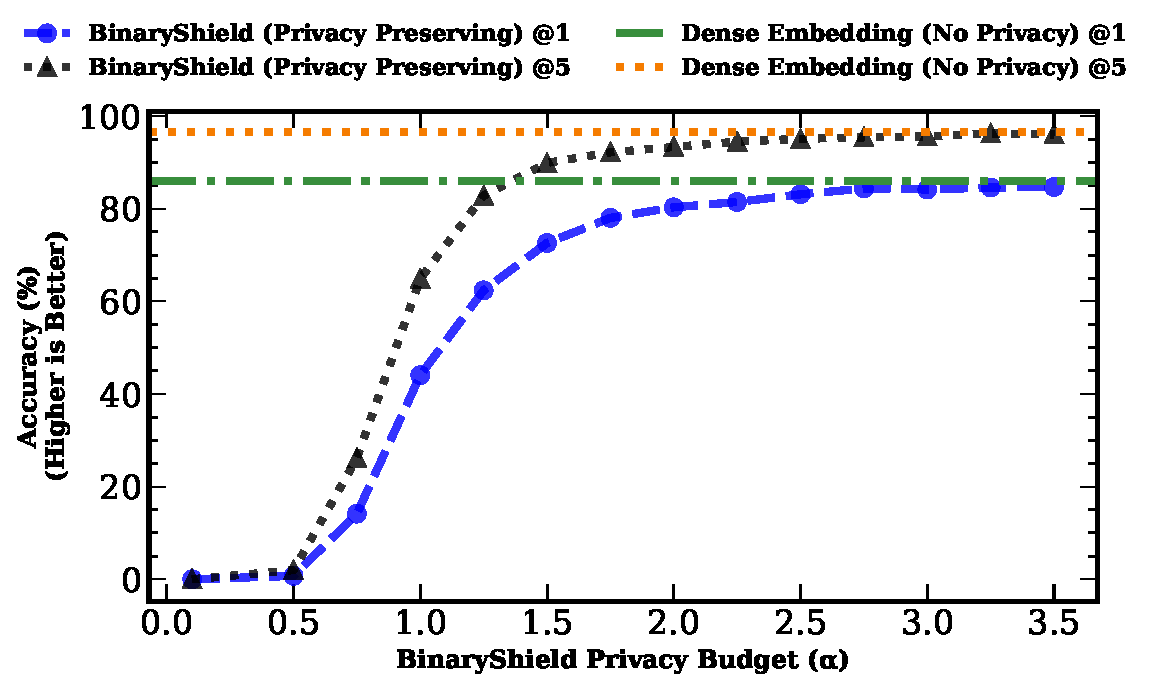
\includegraphics[width=0.8\linewidth]{exp_results/real-world-scenario-results/binaryshield_privacy_utility.pdf}
    \caption{Privacy-utility trade-off for \tool across $\alpha$ values on 50K hybrid corpus.
        Accuracy@1 (blue line) and Accuracy@5 (black line) show phase transition behavior as privacy budget increases.% The non-private dense embedding baseline is shown as horizontal green and orange lines at 86.04\% (Accuracy@1) and 96.56\% (Accuracy@5) respectively.
        }
    \label{fig:Scalability-Privacy--Utility-Trade-off-Characterization}
    \vspace{-4mm}  
\end{figure}


The relationship between privacy protection and threat detection utility at scale represents a fundamental tension in the cross-boundary threat intelligence system.
Similar to Section~\ref{sec:empirical-randomized-response}, to characterize this trade-off precisely, we evaluate \tool's performance across a spectrum of privacy budgets ($\alpha$) on a fixed 50K-entry hybrid corpus containing both malicious prompts and benign WildChat interactions (Section~\ref{sec:large-scale-threat-intelligence-scalability}).
The privacy parameter $\alpha$ directly controls the randomized response mechanism through the bit preservation probability $p = e^{\alpha}/(e^{\alpha} + 1)$, with the corresponding bit flip probability being $1 - p$.
Smaller $\alpha$ values provide stronger privacy guarantees by increasing the probability of bit flips in the binary fingerprint, while larger values preserve more semantic information at the cost of reduced privacy protection.

Our experimental results, visualized in Figure~\ref{fig:Scalability-Privacy--Utility-Trade-off-Characterization}, reveal a sharp phase transition in detection accuracy as the privacy budget increases from highly restrictive to meaningful protective settings. The X-axis represents the privacy parameter $\alpha$, while the Y-axis shows correlation accuracy (Accuracy@1 and Accuracy@5) for both \tool and the \emph{non-private} dense embedding baseline.

At extreme privacy levels ($\alpha = 0.1$), the bit flip probability reaches 0.475, meaning nearly half of all bits are randomly inverted, effectively reducing fingerprints to near-random noise.
Consequently, Accuracy@1 drops to 0\%, rendering threat correlation impossible.
This represents the theoretical limit where maximal privacy completely eliminates utility. As we relax the privacy constraint the bit flip probability decreases.
With $\alpha = 0.75$ (bit flip probability 0.32), Accuracy@1 rises to 14.17\% and Accuracy@5 to 26.15\%, marking the onset of effective threat detection.
At $\alpha = 1.0$  \tool to reach 44.06\% Accuracy@1 and 64.90\% Accuracy@5.
While this is roughly half the non-private baseline (86.04\% and 96.56\%), it shows that meaningful threat correlation is feasible even under strong privacy constraints.
Between $\alpha = 1.0$ and $\alpha = 2.0$, accuracy improves smoothly with meaningful privacy and utility tradefoff.
At $\alpha = 1.25$, Accuracy@1 reaches 62.40\% and Accuracy@5 82.81\%.
At $\alpha = 1.5$, Accuracy@1 is 72.60\% and Accuracy@5 is 89.90\%, retaining 84.4\% of baseline Accuracy@1.


The results show a smooth transition in the privacy-utility trade-off, especially between $\alpha = 0.75$ and $\alpha = 2.0$.
% For high-privacy needs, $\alpha = 1.5$ gives strong privacy. 
Since organizations have already strict security policies, for internal sharing, relaxing privacy to $\alpha = 2.0$--$2.5$ yields near-optimal utility with \emph{realistic} meaningful privacy protection. Overall, \tool potentially can operate in a wide range of privacy-utility trade-offs.

\begin{tcolorbox}[colback=white, colframe=black,  left=0pt, right=0pt, top=0pt, bottom=0pt]
    \textbf{Summary.} \tool empowers organizations to balance privacy and utility as needed, consistently delivering strong accuracy and realistic privacy protection. The organizations can flexibly tune the privacy-utility trade-off based on their operational and regulatory needs.
\end{tcolorbox}

\subsubsection{\tool Computational Efficiency Analysis}
\label{sec:computational-storage-efficiency}

The operational viability of any threat intelligence system fundamentally depends on its ability to process vast quantities of data with minimal latency and storage overhead.
Historical lessons from traditional cybersecurity infrastructure underscore this requirement.
One of the major reasons that signature-based ecosystems (antivirus, IDS) scaled is because compact hashes (e.g., MD5,  fuzzy-hash families).
Similarly, modern LLM services face an even more daunting challenge, processing billions of queries daily across distributed infrastructure.
For \tool to enable practical cross-boundary threat intelligence, it must achieve orders-of-magnitude improvements in both computational speed and storage efficiency compared to \emph{non-private} dense embeddings.
\emph{Every extra byte per fingerprint multiplies into material storage cost, and every millisecond of per-fingerprint scan latency stretches incident response time}.

Figure~\ref{fig:search-time-comparison} reveals \emph{computational advantages} of \tool's fingerprints over dense embeddings. At a corpus size of 10K entries, dense embeddings require 0.87 seconds for similarity search of 968 prompt injections, while \tool completes the same operation in just 0.032 seconds, a 26.7x speedup. This performance gap widens dramatically as corpus size increases. At 100K entries, dense embeddings demand 14.52 seconds, rendering real-time threat correlation infeasible for high-volume services. In contrast, \tool maintains sub-second performance at 0.38 seconds, achieving a 38.1x speedup. The computational efficiency stems from the fundamental difference in similarity computation. Dense embeddings require floating-point dot products or cosine similarity calculations, operations that scale poorly even with optimized linear algebra libraries. \tool's binary fingerprints enable Hamming distance computation through simple XOR operations. We discuss \tool's storage utilization in the appendix. 

\begin{figure}[t]
     \centering
        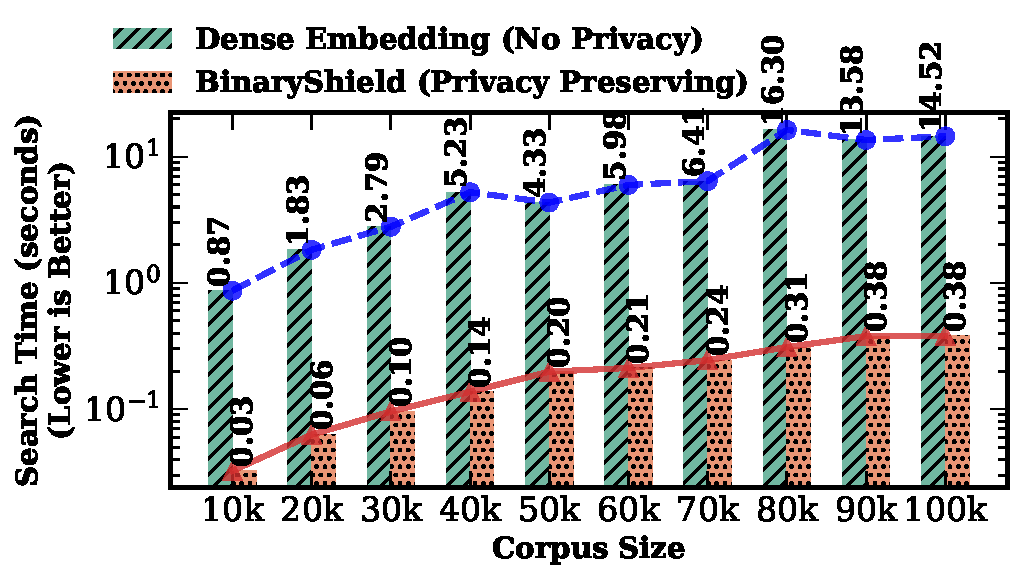
\includegraphics[width=0.7\linewidth]{exp_results/real-world-scenario-results/search_time_scalability_hybrid.pdf}
        \caption{Search time comparison between non-private dense embeddings and \tool across corpus sizes. Note the logarithmic scale on the Y-axis. \tool maintains sub-second performance, demonstrating its suitability for real-time threat correlation at enterprise scale.}
        \label{fig:search-time-comparison}
        \vspace{-4mm}  
\end{figure}



\emph{The practical implications of these efficiency gains extend beyond raw performance metrics (Section ~\ref{sec:comparison-baseline} and ~\ref{sec:large-scale-threat-intelligence-scalability}).}
Consider an organization processing 100 million queries daily across ten services. With dense embeddings, maintaining a rolling 30-day threat intelligence window would require approximately 7.1 TB of storage per boundary and dedicated \emph{GPU clusters} for similarity search making it near to impractical choice. \tool reduces this to 111 GB per boundary, fitting comfortably in memory on commodity servers while enabling CPU-based similarity search. This efficiency democratizes threat intelligence capabilities, allowing even resource-constrained services to participate in collaborative defense without significant infrastructure investment.

Furthermore, the computational efficiency enables new operational capabilities. 
Security teams can now perform retrospective threat hunting across months of historical data in minutes rather than hours.
The reduced storage footprint also facilitates comprehensive threat intelligence archival, enabling long-term trend analysis and attribution of persistent attack campaigns that evolve over extended periods.

\begin{tcolorbox}[colback=white, colframe=black,  left=0pt, right=0pt, top=0pt, bottom=0pt]
    \textbf{Summary.} \tool's computational and storage efficiency fundamentally transforms cross-boundary threat intelligence economics. 
    By reducing search latency up to 38x and storage requirements while maintaining 93\% of non-private baseline top-1 accuracy with privacy, \tool enables enterprise-scale threat correlation. 
    This positions \tool as a practical foundation for collaborative threat intelligence systems against prompt injection attacks. 
\end{tcolorbox}
